\chapter{Abbildungen, Tabellen, Quellcode}
\label{cha:Abbildungen}

\section{Allgemeines}

Abbildungen (\emph{figures}) und Tabellen (\emph{tables}) werden üblicherweise
zusammen mit einem nummerierten Titel (\emph{caption}) zentriert
angeordnet (siehe Abb.~\ref{fig:CocaCola}).
Im Text \emph{muss} es zu jeder Abbildung einen Verweis geben und die eigentliche Abbildung
sollte erst \emph{nach} dem ersten Verweis platziert werden.

\begin{figure}
\centering
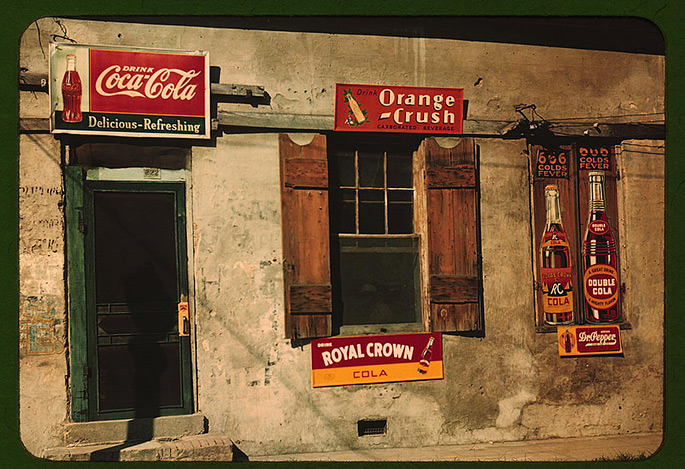
\includegraphics[width=.75\textwidth]{cola-public-domain-photo-p} %{CS0031}
\caption{Coca-Cola Werbung 1940 \cite{CocaCola1940}.}
\label{fig:CocaCola}
\end{figure}



\section{\emph{Let Them Float!}}

Das Platzieren von Abbildungen und Tabellen gehört zu den
schwierigsten Aufgaben im Schriftsatz, weil diese meist viel Platz
benötigen und häufig nicht auf der aktuellen Seite im laufenden
Text untergebracht werden können. Diese Elemente müssen daher an
eine geeignete Stelle auf nachfolgenden Seiten verschoben werden,
was manuell sehr mühsam (jedoch in \emph{Word} beispielsweise unerlässlich) ist.

In \latex funktioniert das weitgehend automatisch, indem
Abbildungen, Tabellen und ähnliche als "`Floating Bodies"'
behandelt werden. Bei der Positionierung dieser Elemente wird
versucht, einerseits im Textfluss möglichst wenig Leer\-raum
entstehen zu lassen und andererseits die Abbildungen und Tabellen
nicht zu weit von der ursprünglichen Textstelle zu entfernen.

Der Gedanke, dass etwa Abbildungen kaum jemals genau an der
ge\-wünsch\-ten Stelle und möglicherweise nicht einmal auf
derselben Seite Platz finden, ist für viele Anfänger aber offenbar sehr
ungewohnt oder sogar beängstigend. Dennoch sollte zunächst einmal
getrost \latex\ diese Arbeit überlassen und \emph{nicht} manuell
eingegriffen werden. Erst am Ende, wenn das gesamte Dokument "`steht"' und
die automatische Platzierung wirklich nicht zufriedenstellend erscheint, sollte (durch gezielte Platzierungsanweisungen
\cite[S.~49]{Oetiker2015}) \textbf{in Einzelfällen} eingegriffen werden.



\section{Captions}

Bei Abbildungen steht der Titel üblicherweise \emph{unten}, bei
Tabellen hingegen -- je nach Konvention -- \emph{oben} (wie in diesem Dokument) 
oder ebenfalls \emph{unten}. In \latex\ erfolgt
auch die Nummerierung der Abbildungen automatisch, ebenso der
Eintrag in das (optionale)
Abbildungsverzeichnis%
\footnote{Ein eigenes Verzeichnis der Abbildungen am Anfang des Dokuments
ist zwar leicht erstellt, in einer Abschlussarbeit aber (und eigentlich
überall sonst auch) überflüssig. Man sollte es daher weglassen.}
am Beginn des Dokuments.

Die Markierung der Captions%
\footnote{Ausnahmsweise wird das Wort "`Caption"' im Folgenden
ohne deutsche Übersetzung verwendet.} erfolgt in \latex mithilfe
der \verb!\label{}! Anweisung, die unmittelbar auf die
\verb!\caption{}! Anweisung folgen muss:
%
\begin{LaTeXCode}[numbers=none]
\begin{figure}
\centering
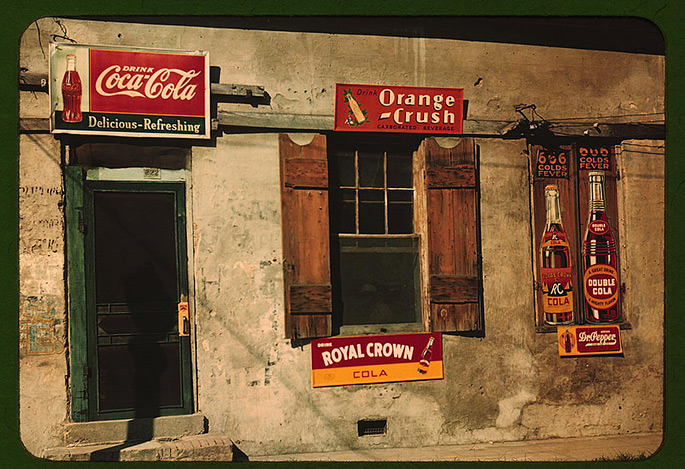
\includegraphics[width=.95\textwidth]{cola-public-domain-photo-p}
\caption{Coca-Cola Werbung 1940 \cite{CocaCola1940}.}
\label{fig:CocaCola}
\end{figure}
\end{LaTeXCode}
%
Der Name des Labels (\texttt{fig:CocaCola}) kann beliebig gewählt werden. 
Die Kennzeichnung \texttt{fig:} ist (wie in Abschn.\ \ref{sec:querverweise} 
erwähnt) nur eine nützliche Hilfe, um beim Schreiben verschiedene Arten 
von Labels besser unterscheiden zu können.

Die Länge der Captions kann dabei sehr unterschiedlich sein. Je
nach Anwendung und Stil ergibt sich manchmal eine sehr kurze
Caption (Abb.~\ref{fig:CocaCola}) oder eine längere
(Abb.~\ref{fig:ibm360}).
Man beachte, wie bei kurzen Captions ein
zentrierter Satz und bei langen Captions ein Blocksatz verwendet
wird (\latex macht das automatisch).
Captions sollten \emph{immer} mit einem Punkt abgeschlossen sein.%
\footnote{Kurioserweise verlangen manche Anleitungen
genau das Gegenteil, angeblich, weil beim klassischen Bleisatz 
die abschließenden Punkte im Druck häufig "`weggebrochen"' sind. 
Das kann man glauben oder nicht, im Digitaldruck 
spielt es jedenfalls keine Rolle.}

\begin{figure}
\centering
\fbox{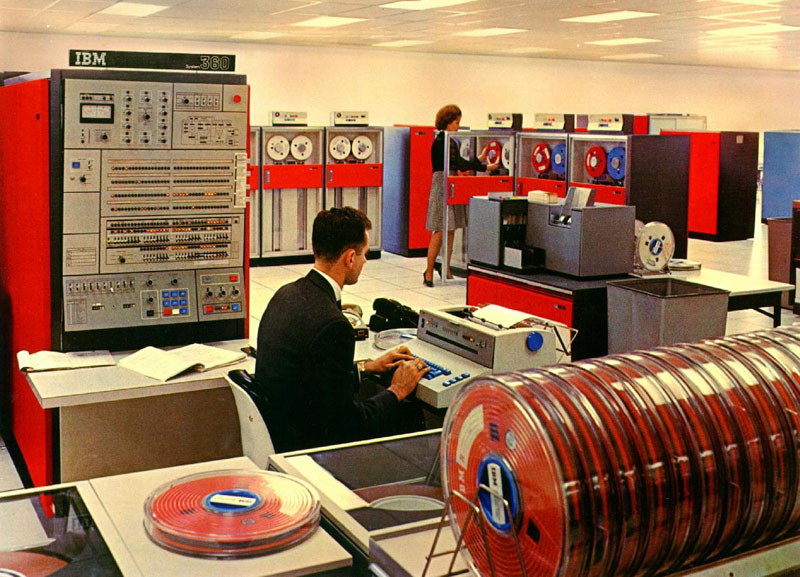
\includegraphics[width=.85\textwidth]{ibm-360-color}}  %{CS1065}}
%\FramePic{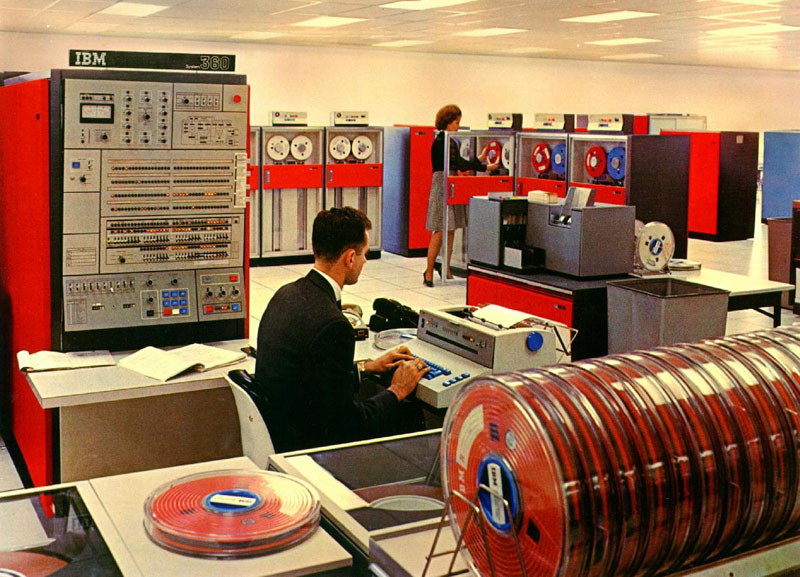
\includegraphics[width=.85\textwidth]{ibm-360-color}} 
\caption{Beispiel für einen langen Caption-Text. \textsc{Univac}
brachte 1961 mit dem Modell 751 den ersten Hochleistungsrechner
mit Halbleiterspeicher auf den Markt. Von diesem Computer wurden
in den U.S.A.\ bereits im ersten Produktionsjahr über fünfzig
Exemplare verkauft, vorwiegend an militärische Dienststellen,
Versicherungen und Großbanken. Die Ablöse erfolgte zwei Jahre
später durch das zusammen mit \textsc{Sperry} entwickelte Modell 820.
Das klingt vielleicht plausibel, ist aber völliger Unsinn, und das
Bild zeigt in Wirklichkeit eine System/360 Anlage von IBM. 
Bildquelle~\cite{IBM360}.} 
\label{fig:ibm360}
\end{figure}





\section{Abbildungen}

Für die Einbindung von Grafiken in \latex wird die Verwendung des Stan\-dard-Pakets
\texttt{graphicx} \cite{Carlisle2016} empfohlen 
(wird durch das \texttt{hagenberg}-Paket bereits eingebunden). 
Mit dem aktuell verwendeten Workflow (\texttt{pdflatex})
können Bild- bzw.\ Grafikformate ausschließlich 
in folgenden Formaten eingebunden werden:
%
\begin{itemize}
	\item \textbf{PNG}: für Grau-, S/W- und Farb-Rasterbilder (bevorzugt),
	\item \textbf{JPEG}: für Fotos (wenn nicht anders vorhanden),
	\item \textbf{PDF}: für Vektorgrafiken (Illustrationen, Strichzeichnungen etc.).
\end{itemize}
%
Bei Rasterbildern sollte wenn möglich PNG verwendet werden, weil die darin 
enthaltenen Bilder verlustfrei komprimiert sind und daher keine sichtbaren Kompressionsartefakte
aufweisen. Im Gegensatz dazu sollte JPEG nur dann verwendet werden, wenn das Originalmaterial
(Foto) bereits in dieser Form vorliegt.


\subsection{Wo liegen die Grafikdateien?} 

Die Bilder werden üblicherweise in einem Unterverzeichnis (oder in mehreren Unterverzeichnissen) abgelegt,
im Fall dieses Dokuments in \nolinkurl{images/}.
Dazu dient die folgende Anweisung
am Beginn des Hauptdokuments \nolinkurl{_DaBa.tex} (\sa\ Anhang \ref{app:latex}):
%
\begin{quote}
\verb!\graphicspath{{images/}}!
\end{quote}
%
Der (zum Hauptdokument relative) Pfad \texttt{graphicspath} kann innerhalb des
Dokuments jederzeit geändert werden, was durchaus nützlich ist, wenn
\zB\ die Grafiken einzelner Kapitel getrennt in entsprechenden Verzeichnissen
abgelegt werden sollen.
Die Größe der Abbildung im Druck kann durch Vorgabe einer bestimmten
Breite oder Höhe oder eines Skalierungsfaktors gesteuert werden, {\zB}:
%
\begin{quote}
\verb!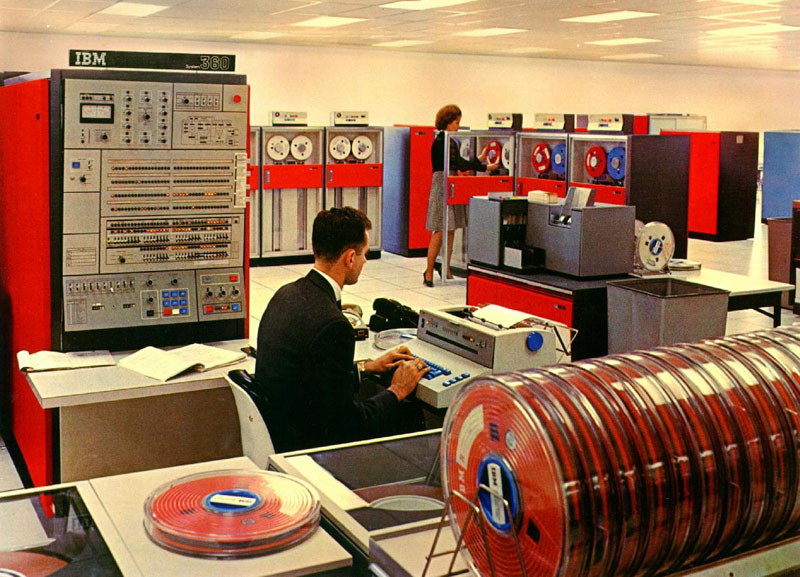
\includegraphics[width=.85\textwidth]{ibm-360-color}! \\
\verb!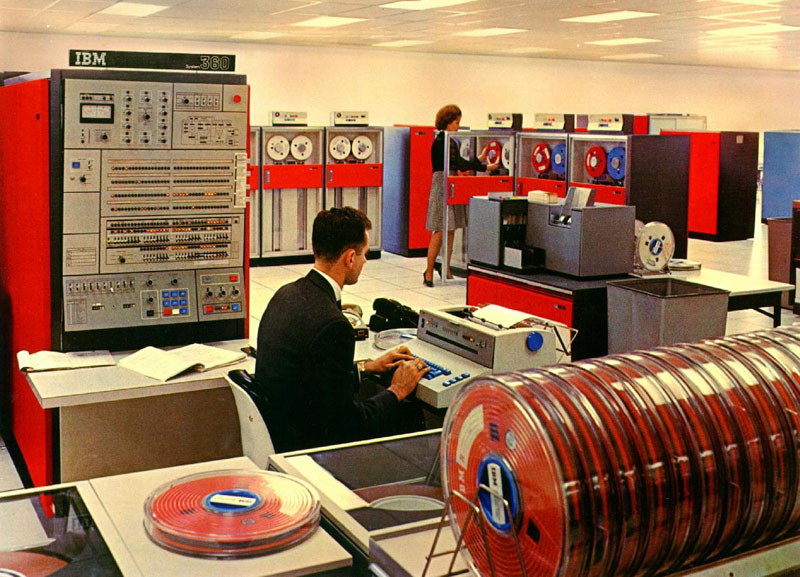
\includegraphics[scale=1.5]{ibm-360-color}!
\end{quote}
%
Man beachte, dass dabei die Dateiendung nicht explizit angegeben werden muss. 
Das ist \va\ dann praktisch, wenn verschiedene Workflows mit jeweils
unterschiedlichen Dateitypen verwendet werden.


\subsection{Grafiken einrahmen} 

%Mit dem Makro \verb!\FramePic{}! (definiert in \texttt{hgb.sty}) kann optional ein dünner 
%Rahmen rund um die Grafik erzeugt werden, \zB:
Mit dem Makro \verb!\fbox{...}! kann optional ein dünner 
Rahmen rund um die Grafik erzeugt werden, \zB:
%
\begin{quote}
%\verb!\FramePic{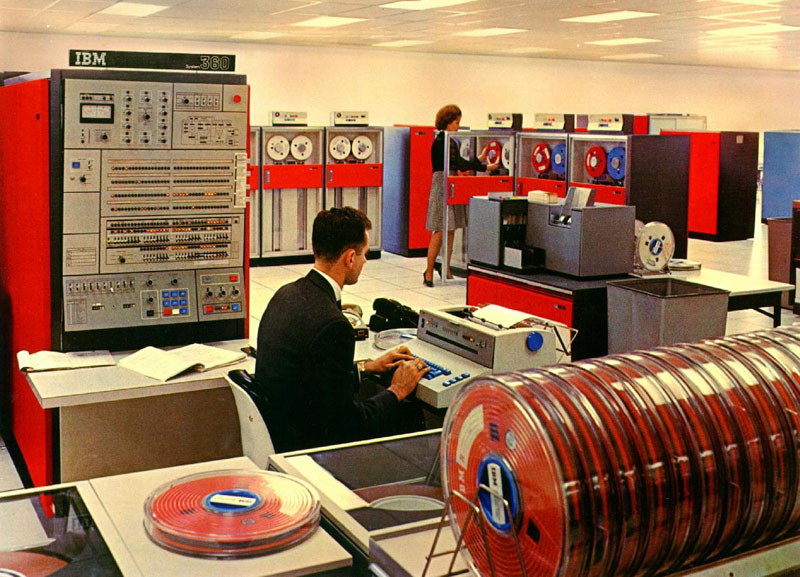
\includegraphics[height=50mm]{ibm-360-color}}!
\verb!\fbox{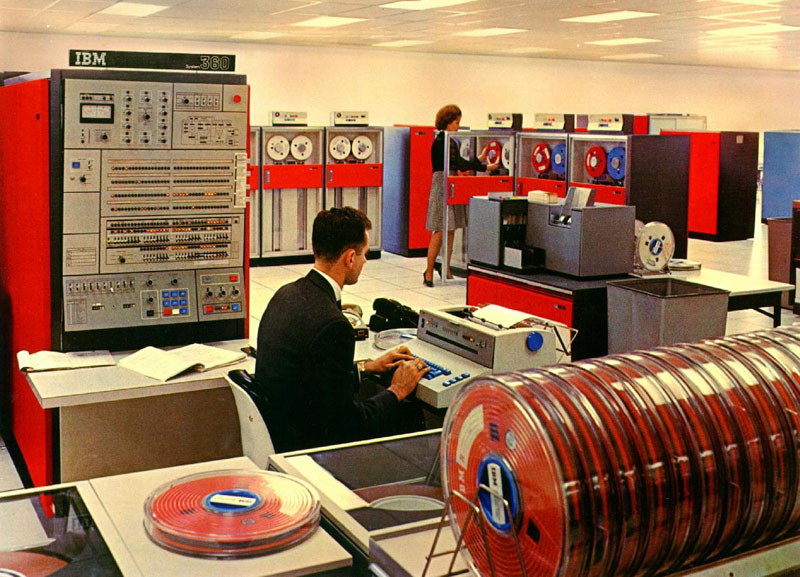
\includegraphics[height=50mm]{ibm-360-color}}!
\end{quote}
%
Das wird üblicherweise nur bei Rasterbildern nötig sein, insbesondere wenn sie zum Rand hin sehr hell sind
und ohne Rahmen nicht vom Hintergrund abgrenzbar wären.

\subsection{Rasterbilder (Pixelgrafiken)}

Generell sollten Bilder bereits vorher so aufbereitet werden,
dass sie später beim Druck möglichst wenig an Qualität verlieren.
Es empfiehlt sich daher, die Bildgröße (Auflösung) bereits im Vorhinein
(\zB mit \emph{Photoshop})
richtig einzustellen.
Brauchbare Auflösungen bezogen auf die endgültige Bildgröße sind:
%
\begin{itemize}
  \item \textbf{Farb- und Grauwertbilder:} 150--300 dpi
  \item \textbf{Binärbilder (Schwarz/Weiß):} 300--600 dpi
\end{itemize}
%
Eine wesentlich höhere Auflösung macht aufgrund der beim Laserdruck notwendigen
Rasterung keinen Sinn, auch bei 1200 dpi-Druckern.
Speziell \emph{Screen\-shots} sollten nicht zu klein dargestellt werden,
da sie sonst schlecht lesbar sind (max.\ 200 dpi, besser 150 dpi).
Dabei ist zu bedenken, dass die Arbeit auch als Kopie in allen
Details noch gut lesbar sein sollte.

\subsubsection{JPEG-Problematik}

In der Regel sollten Bilder, die für den Einsatz in
Druckdokumenten gedacht sind, nicht mit verlustbehafteten
Kompressionsverfahren abgespeichert werden. Insbesondere sollte die Verwendung
von JPEG möglichst vermieden werden, auch wenn viele Dateien dadurch
wesentlich kleiner werden. 
Eine Ausnahme ist, wenn die Originaldaten nur in JPEG vorliegen und für die 
Einbindung nicht bearbeitet oder verkleinert wurden. Ansonsten sollte immer
PNG verwendet werden.

Besonders gerne werden farbige \textbf{Screenshots} einer JPEG-Kompression%
\footnote{Das JPEG-Verfahren ist für natürliche Fotos konzipiert und dafür auch gut geeignet,
seine undifferenzierte Verwendung ist aber zu einer globalen Plage geworden.}
unterzogen, obwohl deren verheerende Folgen für jeden Laien sichtbar sein sollten
(Abb.~\ref{fig:jpeg-pfusch}).

\begin{figure}
\centering\small
\begin{tabular}{cc}
%\FramePic{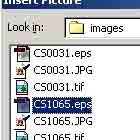
\includegraphics[width=0.45\textwidth]{screenshot-dirty}} &		% JPEG file
%\FramePic{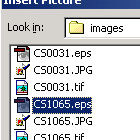
\includegraphics[width=0.45\textwidth]{screenshot-clean}} \\	% PNG file
\fbox{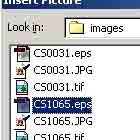
\includegraphics[width=0.45\textwidth]{screenshot-dirty}} &		% JPEG file
\fbox{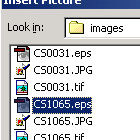
\includegraphics[width=0.45\textwidth]{screenshot-clean}} \\	% PNG file
(a) & (b) 
\end{tabular}
\caption{Typischer JPEG-Pfusch. Screenshots und ähnliche im Original
verfügbare Rasterbilder sollten für Druckdokumente \emph{keinesfalls} mit
JPEG komprimiert werden. Das Ergebnis~(a) sieht gegenüber dem
unkomprimierten Original~(b) nicht nur schmutzig aus, sondern wird
im Druck auch schnell unleserlich.} 
\label{fig:jpeg-pfusch}
\end{figure}



\subsection{Vektorgrafiken}

Für schematische Abbildungen (\zB Flussdiagramme, Entity-Relationship-Diagramme
oder sonstige strukturelle Darstellungen) sollten unbedingt
Vektorgrafiken (PDF) verwendet werden. % (\zB Abb.~\ref{fig:latex-pdf-workflow}).
Gerasterte Grafiken, wie sie üblicherweise als GIF- oder PNG-Dateien
auf Webseiten vorliegen, haben in einem Druckdokument nichts zu suchen, notfalls
müssen sie mit einem entsprechenden Werkzeug \emph{neu} gezeichnet werden (natürlich
unter Angabe der ursprünglichen Quelle).

In diesem Fall kommt als Datenformat nur PDF %(oder EPS im DVI-PS-Workflow) 
in Frage,
dieses bietet sich aber auch in anderen Umgebungen als universelles
Vektor-Format an.
Zur Erstellung von PDF-Vektorgrafiken wird ein geeignetes
Grafikprogramm, \zB\ %\emph{Freehand} von \emph{Macromedia} oder
\emph{Illustrator} von \emph{Adobe} benötigt.
Manche gängigen Grafikprogramme 
unterstützen allerdings keinen direkten Export von PDF-Dateien
oder erzeugen unsaubere Dateien. Vor der Entscheidung
für eine bestimmte Zeichensoftware sollte das im Zweifelsfall
ausprobiert werden.
PDF kann im Notfall über einen entsprechenden Druckertreiber erzeugt werden.


\subsubsection{Vektorgrafiken mit \emph{Inkscape}}
\label{sec:InkscapeGraphics}

Mit \emph{Inkscape}\footnote{\url{https://inkscape.org/}} können Vektorgrafiken auf
sehr einfache Weise erstellt werden.
Das Basisformat von Inkscape ist SVG,
nach dem Export als PDF können solche Grafiken aber wie üblich mit
\verb!\includegraphics[..]{..}! in \latex\ eingefügt werden.

Eine interessante Möglichkeit dabei ist, Texte innerhalb der Grafik
durch \latex\ automatisch ersetzen zu lassen.
Dadurch werden in der fertigen Grafik dieselben Schriften wie im Fließtext
verwendet und \va\ mathematische Elemente entsprechend ersetzt.
Abbildung \ref{fig:InkscapeExample} zeigt ein Beispiel dazu:
%
\begin{itemize}
\item
Die ursprüngliche Inkscape-Grafik \nolinkurl{images/inkscape-template.svg}  enthält
Texte, die nachträglich von \latex\ ersetzt werden sollen 
(siehe Abb.~\ref{fig:InkscapeExample} (a)).
\item
Durch \textsf{Save a Copy...} (als PDF) in Inkscape, mit den Einstellungen wie in 
Abb.~\ref{fig:InkscapeExample} (c), werden folgende zwei Files erzeugt:
\begin{itemize}
\item[] \nolinkurl{inkscape-template.pdf}: eine PDF-Datei der Grafik ohne Texte, 
\item[] \nolinkurl{inkscape-template.pdf_tex}: eine \latex-Datei mit allen relevanten Informationen.
\end{itemize}
\end{itemize}
%
Die Einbindung der Grafik in das Dokument erfolgt schließlich durch
\begin{itemize}
\item[] \verb!\input{images/inkscape-template.pdf_tex}!,
\end{itemize}
mit dem in Abb.~\ref{fig:InkscapeExample} (b) gezeigten Ergebnis.



\begin{figure}
\centering\small
\begin{tabular}{cc}
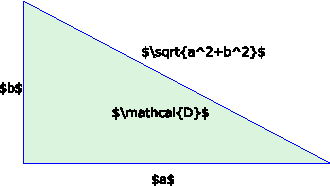
\includegraphics[scale=1.0]{inkscape-template-orig} &
\input{images/inkscape-template.pdf_tex}
\\
(a) & (b)
\\[6pt]
\multicolumn{2}{c}{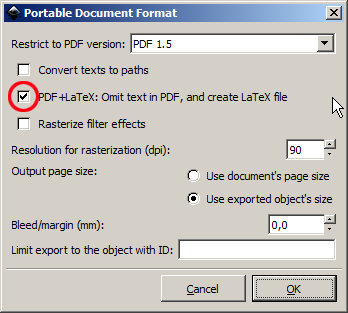
\includegraphics[width=0.4\textwidth]{inkscape-pdf-save-screenhot}%
~~\raisebox{25mm}{(c)}}
\end{tabular}
\caption{Beispiel für eine mit \emph{Inkscape} erzeugte Vektorgrafik
(\nolinkurl{inkscape-template.svg}).
Originalgrafik im \textit{Inkscape}-Editor (a);
beim Einfügen werden die Texte automatisch durch LaTeX ersetzt (b).
Beim Speichern in Inkscape (als PDF) ist auf die Einstellung "`PDF+LaTeX"' zu achten (c).}
\label{fig:InkscapeExample}
\end{figure}


\subsubsection{Einbettung von Schriften}

Die Wiedergabe von Textelementen ist abhängig von der auf dem
Computer (oder Drucker) installierten Schriften und der Form der
Schrifteinbettung im Quelldokument. Die korrekte Darstellung am
Bildschirm eines Computers bedeutet nicht, dass dasselbe Dokument
auf einem anderen Computer oder Drucker genau so dargestellt wird.
Dieser Umstand ist besonders wichtig, wenn Druckdokumente online
zur Verfügung gestellt werden. Kontrollieren Sie daher genau, ob
die innerhalb Ihrer Grafiken verwendeten Schriften auch exakt wie
beabsichtigt im Ausdruck aufscheinen.


\subsubsection{Strichstärken -- \emph{Hairlines} vermeiden!}

In Grafik-Programmen wie \emph{Freehand} und \emph{Illustrator},
die sich im Wesentlichen an der \emph{PostScript}-Funktionalität
orientieren, ist es möglich, Linien bzgl.\ ihrer Stärke als
"`Hairline"' zu definieren. Im zugehörigen \emph{PostScript}-Code
wird dies als \texttt{linewidth} mit dem Wert \texttt{0} ausgedrückt und
sollte am Ausgabegerät "`möglichst dünne"' Linien ergeben. 
Das Ergebnis ist ausschließlich vom jeweiligen Drucker
abhängig und somit kaum vorhersagbar.
\textbf{Fazit:} Hairlines vermeiden und stattdessen immer konkrete
Strichstärken ($\geq 0.25\,\mathrm{pt}$) einstellen!





\subsection{\tex-Schriften auch in Grafiken?}
\label{sec:tex-schriften-in-grafiken}

Während bei Abbildungen, die mit externen
Grafik-Programmen erzeugt werden, meist mit ähnlich aussehende
Schriften (wie \emph{Times-Roman} oder \emph{Garamond}) Abhilfe schaffen,
besteht bei Puristen oft der verständliche Wunsch, die 
\emph{Computer-Modern} (CM) Schriftfamilie von {\tex}/{\latex} auch
innerhalb von eingebetteten Grafiken einzusetzen.

\subsubsection{\emph{BaKoMa}-Schriften (TrueType)}

Glücklicherweise stehen einige Portierungen von CM als {\em
TrueType}-Schriften zur Verfügung, die auch in herkömmlichen
DTP-Anwendungen unter \emph{Windows} und \emph{Mac~OS} verwendet werden
können. Empfehlenswert ist \zB\ die \emph{BaKoMa Fonts
Collection}\footnote{Von Basil K.\ Malyshev -- die BaKoMa-Fonts
liegen dieser Vorlage bei, ansonsten finden sie sich \zB\ unter
\url{www.ctan.org/tex-archive/fonts/cm/ps-type1/bakoma/}.}, die
neben den CM-Standardschriften auch die mathematischen Schriften
der AMS-Familie ent\-hält und zudem kostenfrei ist. Natürlich
müssen die TrueType Schriften vor der Verwendung zunächst auf dem
eigenen PC installiert werden. 
%Ein Beispiel für eine in {\em
%Freehand} erzeugte Grafik mit CM-Schriften findet sich in
%Abb.~\ref{fig:latex-pdf-workflow} (Seite
%\pageref{fig:latex-pdf-workflow}).

\subsubsection{\emph{Latin Modern Roman} Fonts (OpenType)}

Eine Alternative dazu sind die "`LM-Roman"'%
\footnote{\url{http://www.gust.org.pl/projects/e-foundry/latin-modern}}
 Open-Type Schriften, die speziell für die Verwendung im Umfeld von \latex\ entwickelt wurden.
Sie sind auch Teil der MikTeX-Installation.%
\footnote{\zB unter \url{C:/Program Files (x86)/MikTeX 2.9/fonts/opentype/public/lm/}}
Diese Schriften enthalten \ua\ Zeichen mit Umlauten und sind daher auch für deutsche Texte recht
bequem zu verwenden.




\subsection{Für Gourmets: Grafiken mit \latex-Overlays}
\label{sec:GraphicOverlays}

Bisweilen ist es erforderlich, ein bestehendes Bilder oder eine Grafik mit 
\latex-eigenen (Vektor-)Elementen zu überlagern, \zB\ für Markierungen
oder Beschriftungen. Ein typisches Beispiel ist in Abb.~\ref{fig:overpic-example}
gezeigt, wo eine mit \emph{Mathematica} generierte PDF-Grafik
mit mathematischen Elementen annotiert wird.


\begin{figure}
\centering\small
%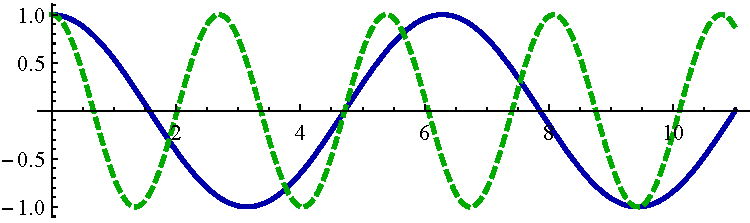
\includegraphics[width=0.85\textwidth]{mathematica-example}
\vspace*{3mm}
\begin{overpic}[width=0.85\textwidth]{mathematica-example}
	\put(101,14){$x$}%
	\put(4,31){$f(x)$}%
	\put(29.5,28){\line(1,1){2}}%
	{\color{green!70!black}\put(29.5,28){\circle*{2.0}}}%
	\put(32,30){$\cos(\frac{7}{3} x)$}%
	\put(59,28){\line(1,1){2}}%
	{\color{blue!70!black}\put(59,28){\circle*{2.0}}}%
	\put(61.5,30){$\cos(x)$}%
\end{overpic}
\caption{Beispiel für die Verwendung des \texttt{overpic}-Pakets zum Einfügen
von \latex-Elementen über eine importierte Grafik.
In diesem Fall wurden die mathematischen Elemente $x$, $f(x)$, $\cos(x)$ und $\smash{\cos(\frac{7}{3} x)}$
sowie zwei diagonale Geraden und gefüllte (färbige) Kreise eingefügt.
Darunter liegt die Vektor\-grafik \texttt{mathematica-example.pdf}.}
\label{fig:overpic-example}
\end{figure}



Dazu wird das \texttt{overpic}-Paket\footnote{\url{https://www.ctan.org/pkg/overpic}}
verwendet und zum Importieren der Grafik anstelle von \verb!\includegraphics!
die Umgebung \verb!\begin{overpic}! \ldots \verb!\end{overpic}! verwendet 
(mit ähnlicher Syntax):

\begin{LaTeXCode}[numbers=none]
\begin{overpic}[width=0.85\textwidth]{mathematica-example}
	\put(101,14){$x$}%
	\put(4,31){$f(x)$}%
	\put(29.5,28){\line(1,1){2}}%
	...
\end{overpic}
\end{LaTeXCode}

Die \texttt{overpic}-Umgebung bildet gleichzeitig eine \texttt{picture}-Umgebung, 
in der \latex-Zeichenanweisungen (wie \verb!\put! u.ä.) platziert werden
können, wie in obigem Beispiel gezeigt.\footnote{Die Standard-Zeichenanweisungen
in \latex sind ziemlich restriktiv, weshalb hier zusätzlich das \texttt{pict2e}-Paket
(\url{https://www.ctan.org/pkg/pict2e}) verwendet wird.}
Die $x/y$-Positionen sind in Prozent der Bildbreite angegeben.
Weitere Details finden sich im Quelltext.





\subsection{Abbildungen mit mehreren Elementen}

Werden mehrere Bilder oder Grafiken zu einer Abbildung zusammengefasst, 
wird üblicherweise eine gemeinsame Caption verwendet, wie in Abb.~\ref{fig:Bearings}
dargestellt. Im Text könnte ein Verweis auf einen einzelnen Teil der Abbildung, etwa das 
einreihige Rollenlager in Abb.~\ref{fig:Bearings} (c), so aussehen:
%
\begin{LaTeXCode}[numbers=none]
    ... Abb.~\ref{fig:Bearings} (c) ... 
\end{LaTeXCode}


\subsection{Quellenangaben in Captions}
\label{sec:QuellenangabenInCaptions}

Wenn Bilder, Grafiken oder Tabellen aus anderen Quellen verwendet werden, dann 
muss ihre Herkunft in jedem Fall klar ersichtlich gemacht werden, und zwar am 
besten direkt in der Caption.
Wird beispielsweise eine Grafik aus einem Buch oder einer sonstigen 
zitierfähigen Publikation verwendet, dann sollte diese in das Literaturverzeichnis 
aufgenommen und wie üblich mit
\verb!\cite{..}! zitiert werden, wie in Abb.\ \ref{fig:Bearings} demonstriert. 
Weitere Details zu dieser Art von Quellenangaben finden sich in 
Kap.\ \ref{cha:Literatur} (insbes.\ Abschnitt \ref{sec:KategorieOnline}).

\begin{figure}
\centering\small
\setlength{\tabcolsep}{0mm}	% alle Spaltenränder auf 0mm
\begin{tabular}{c@{\hspace{12mm}}c} % mittlerer Abstand = 12mm
  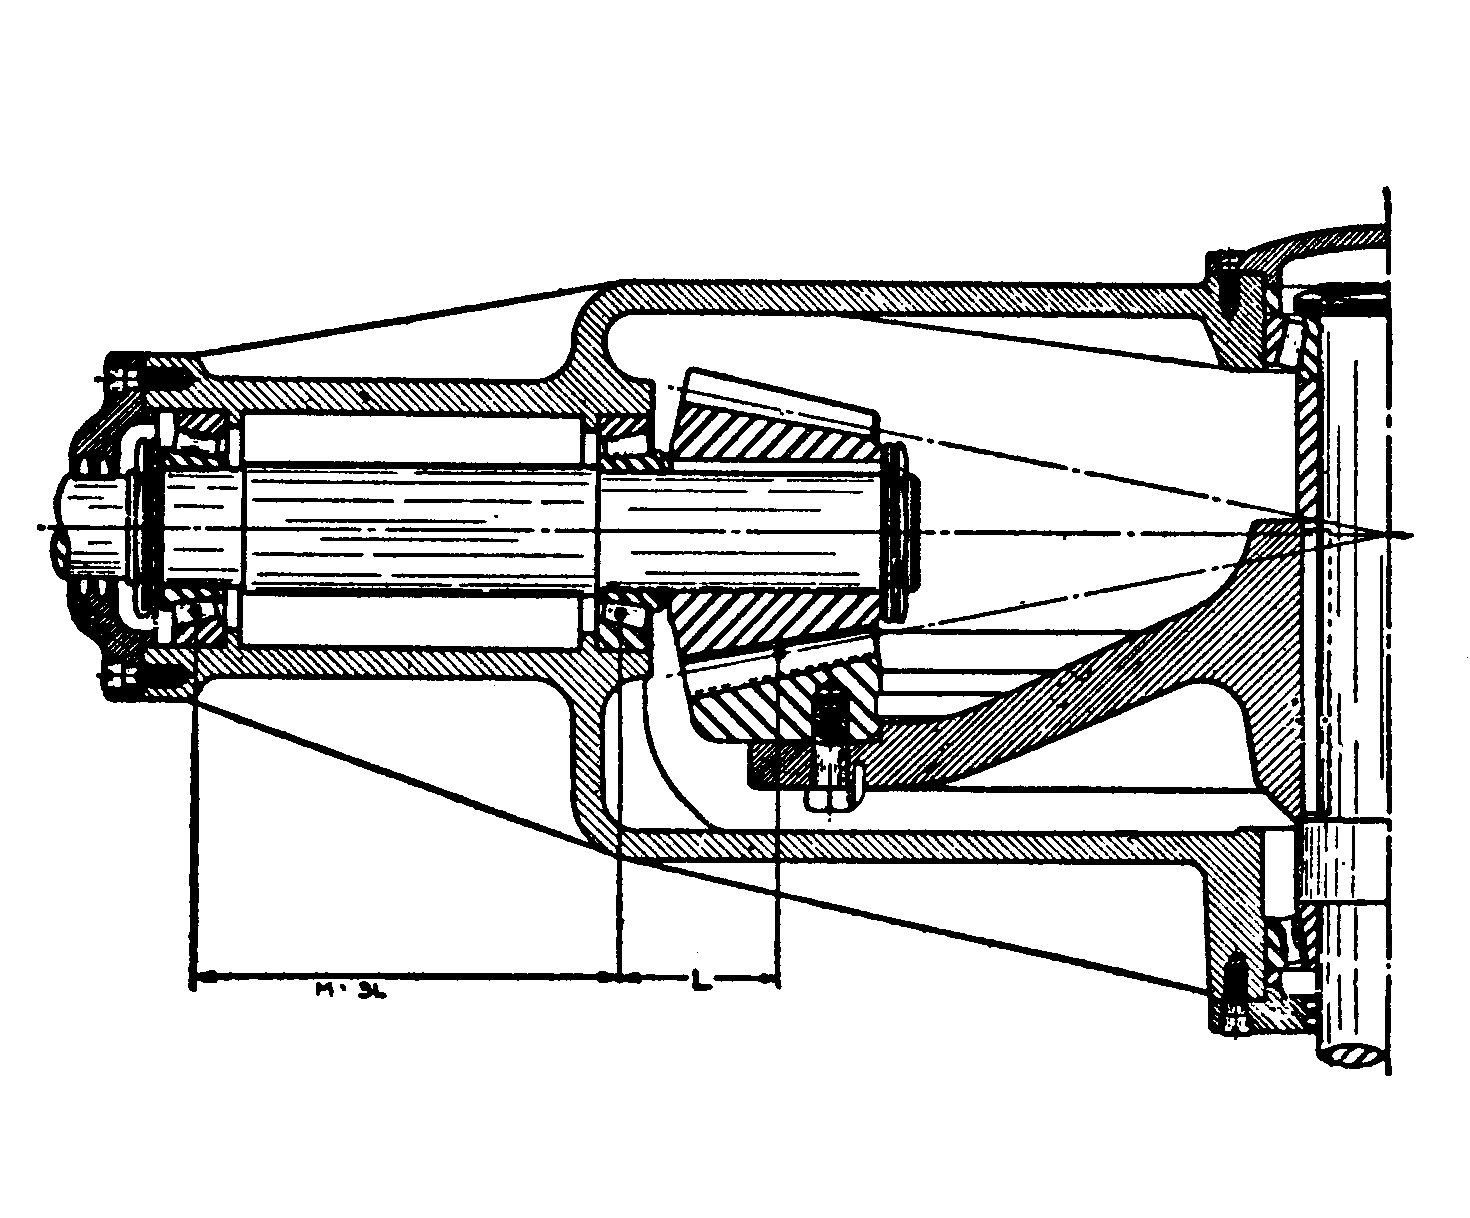
\includegraphics[width=.45\textwidth]{overhang-mounting} &
  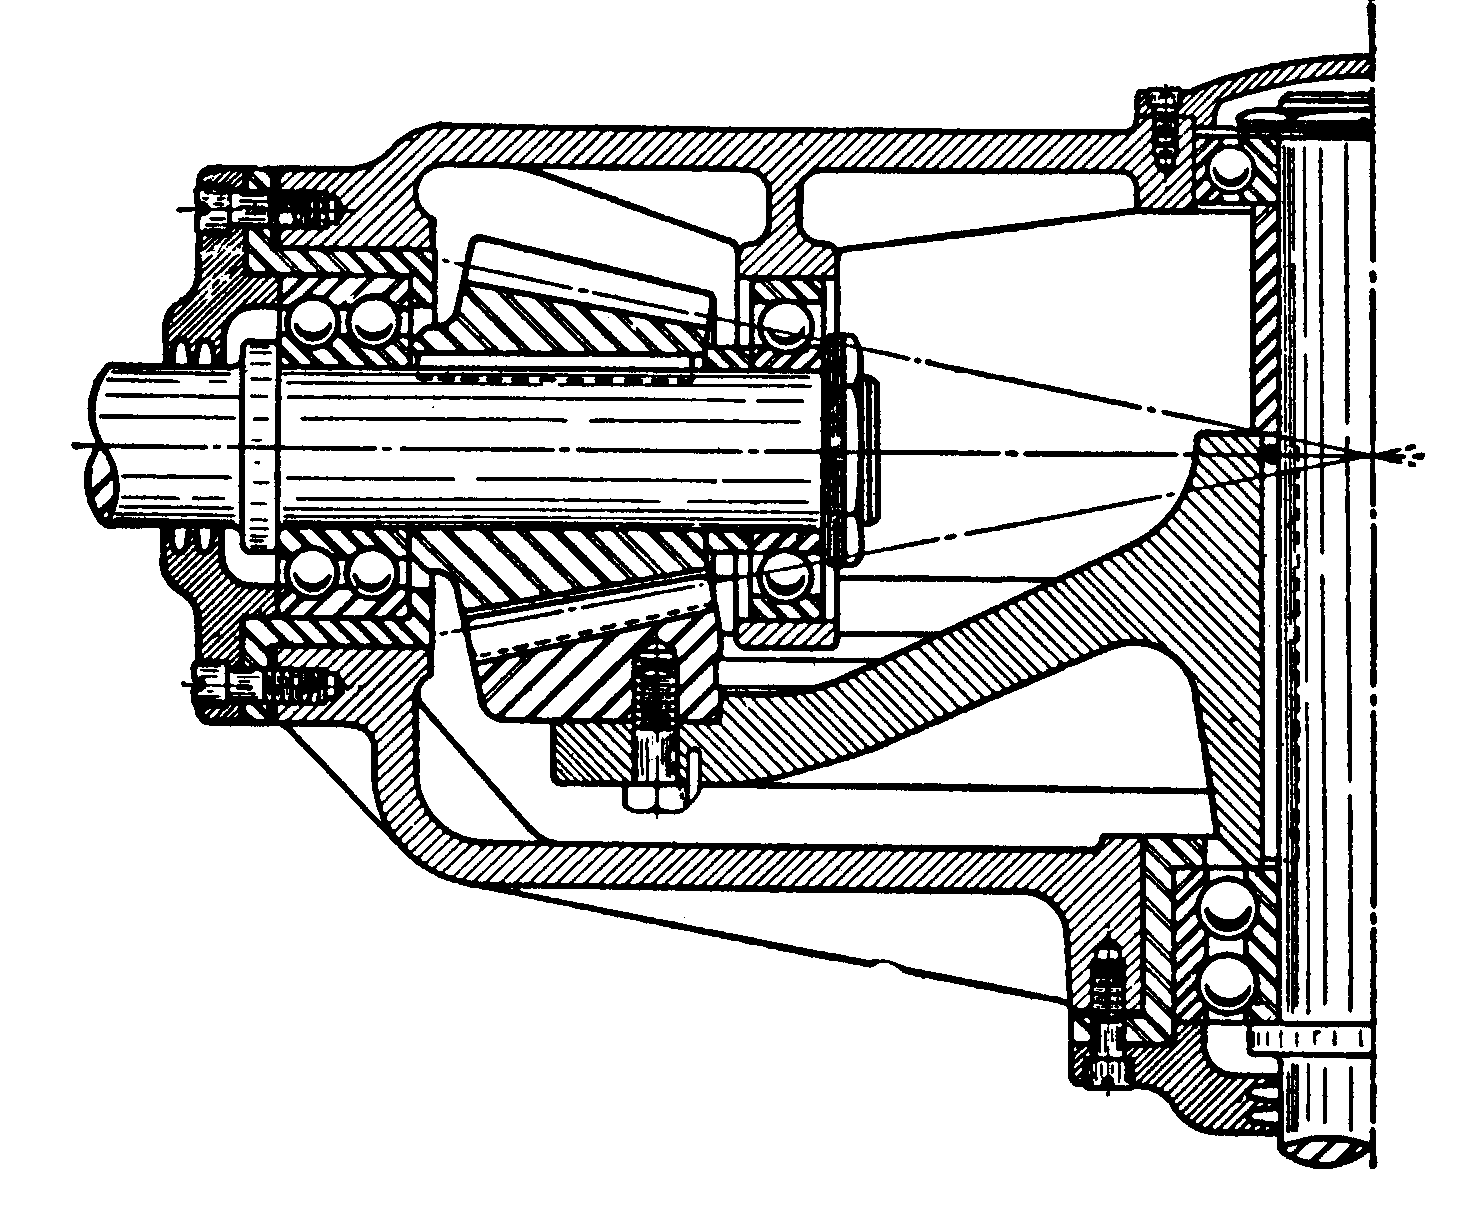
\includegraphics[width=.45\textwidth]{straddle-mounting} 
\\
  (a) & (b)
\\[4pt]	%vertical extra spacing (4 points)
  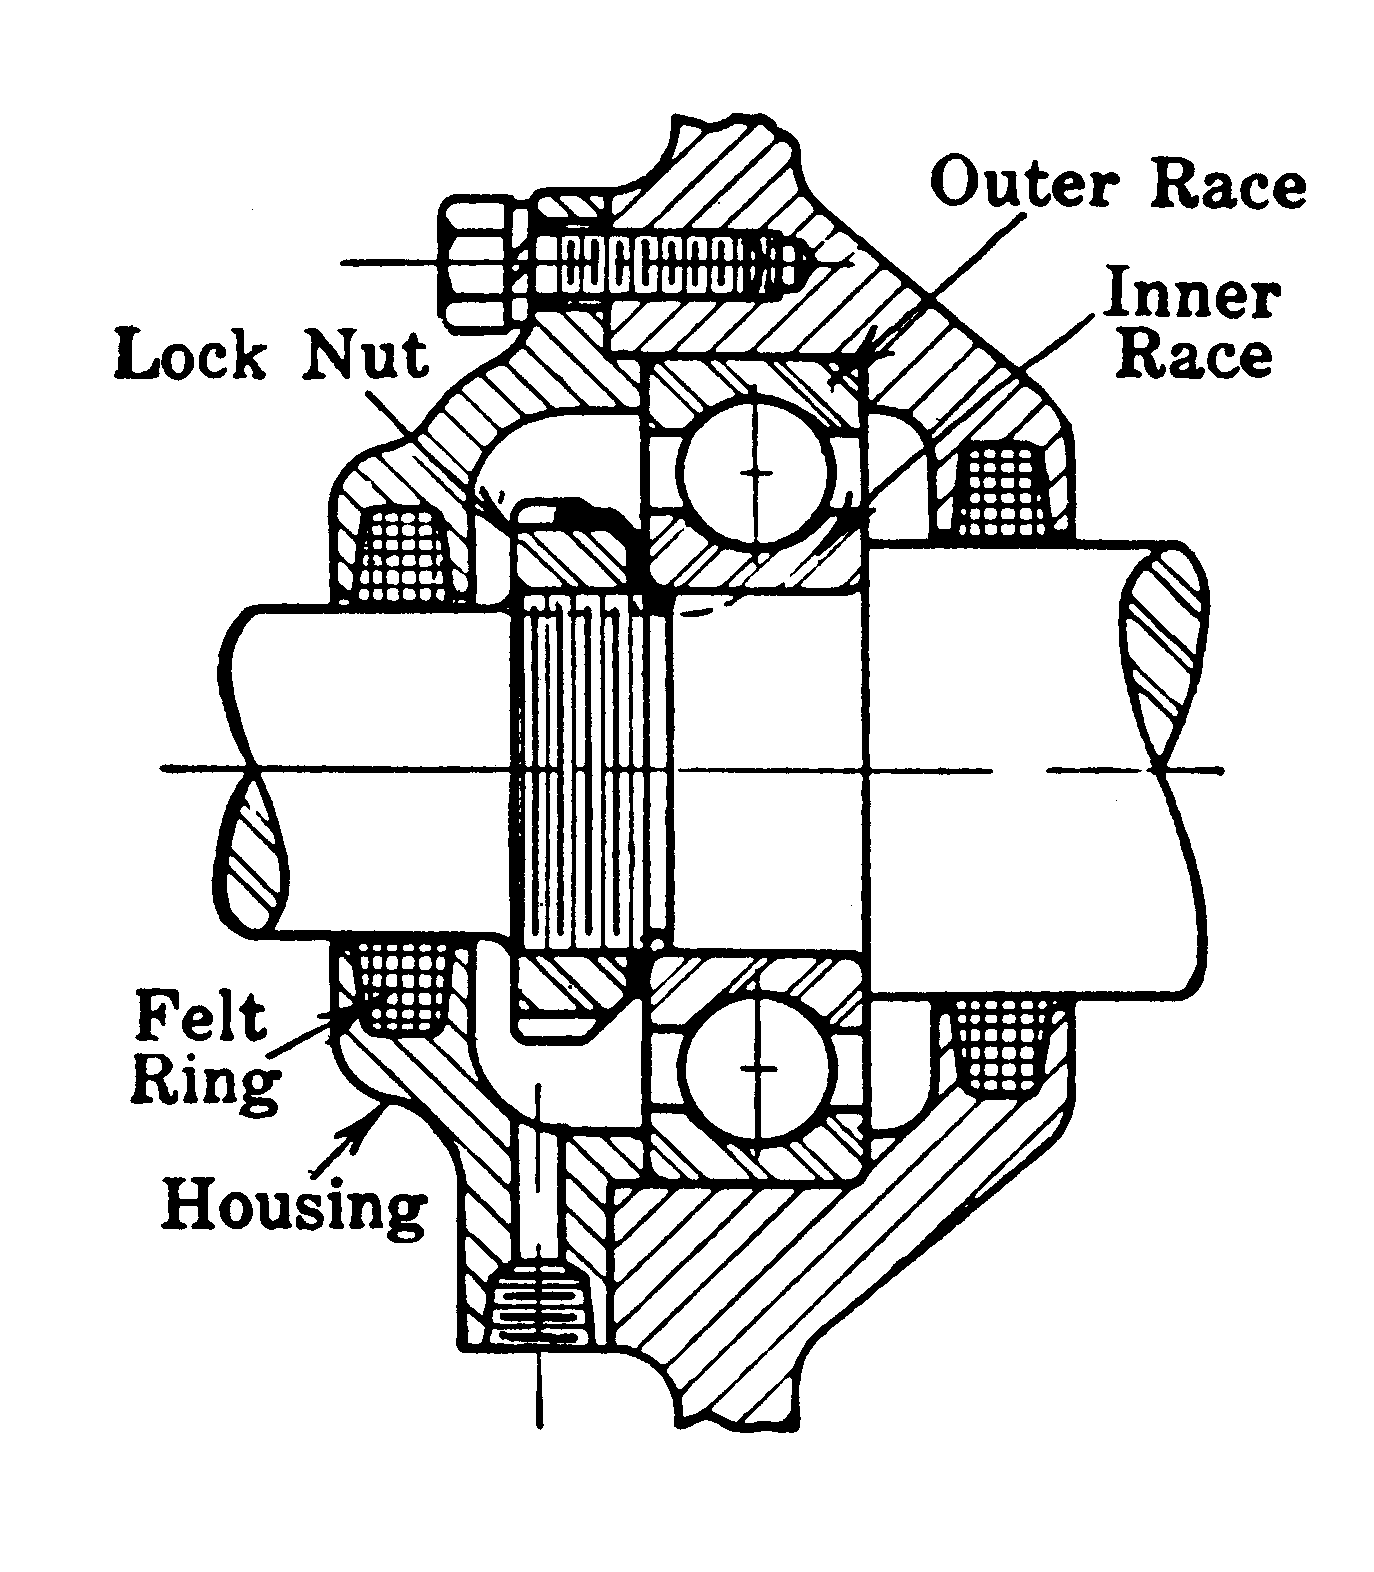
\includegraphics[width=.45\textwidth]{ball-bearing-1} &
  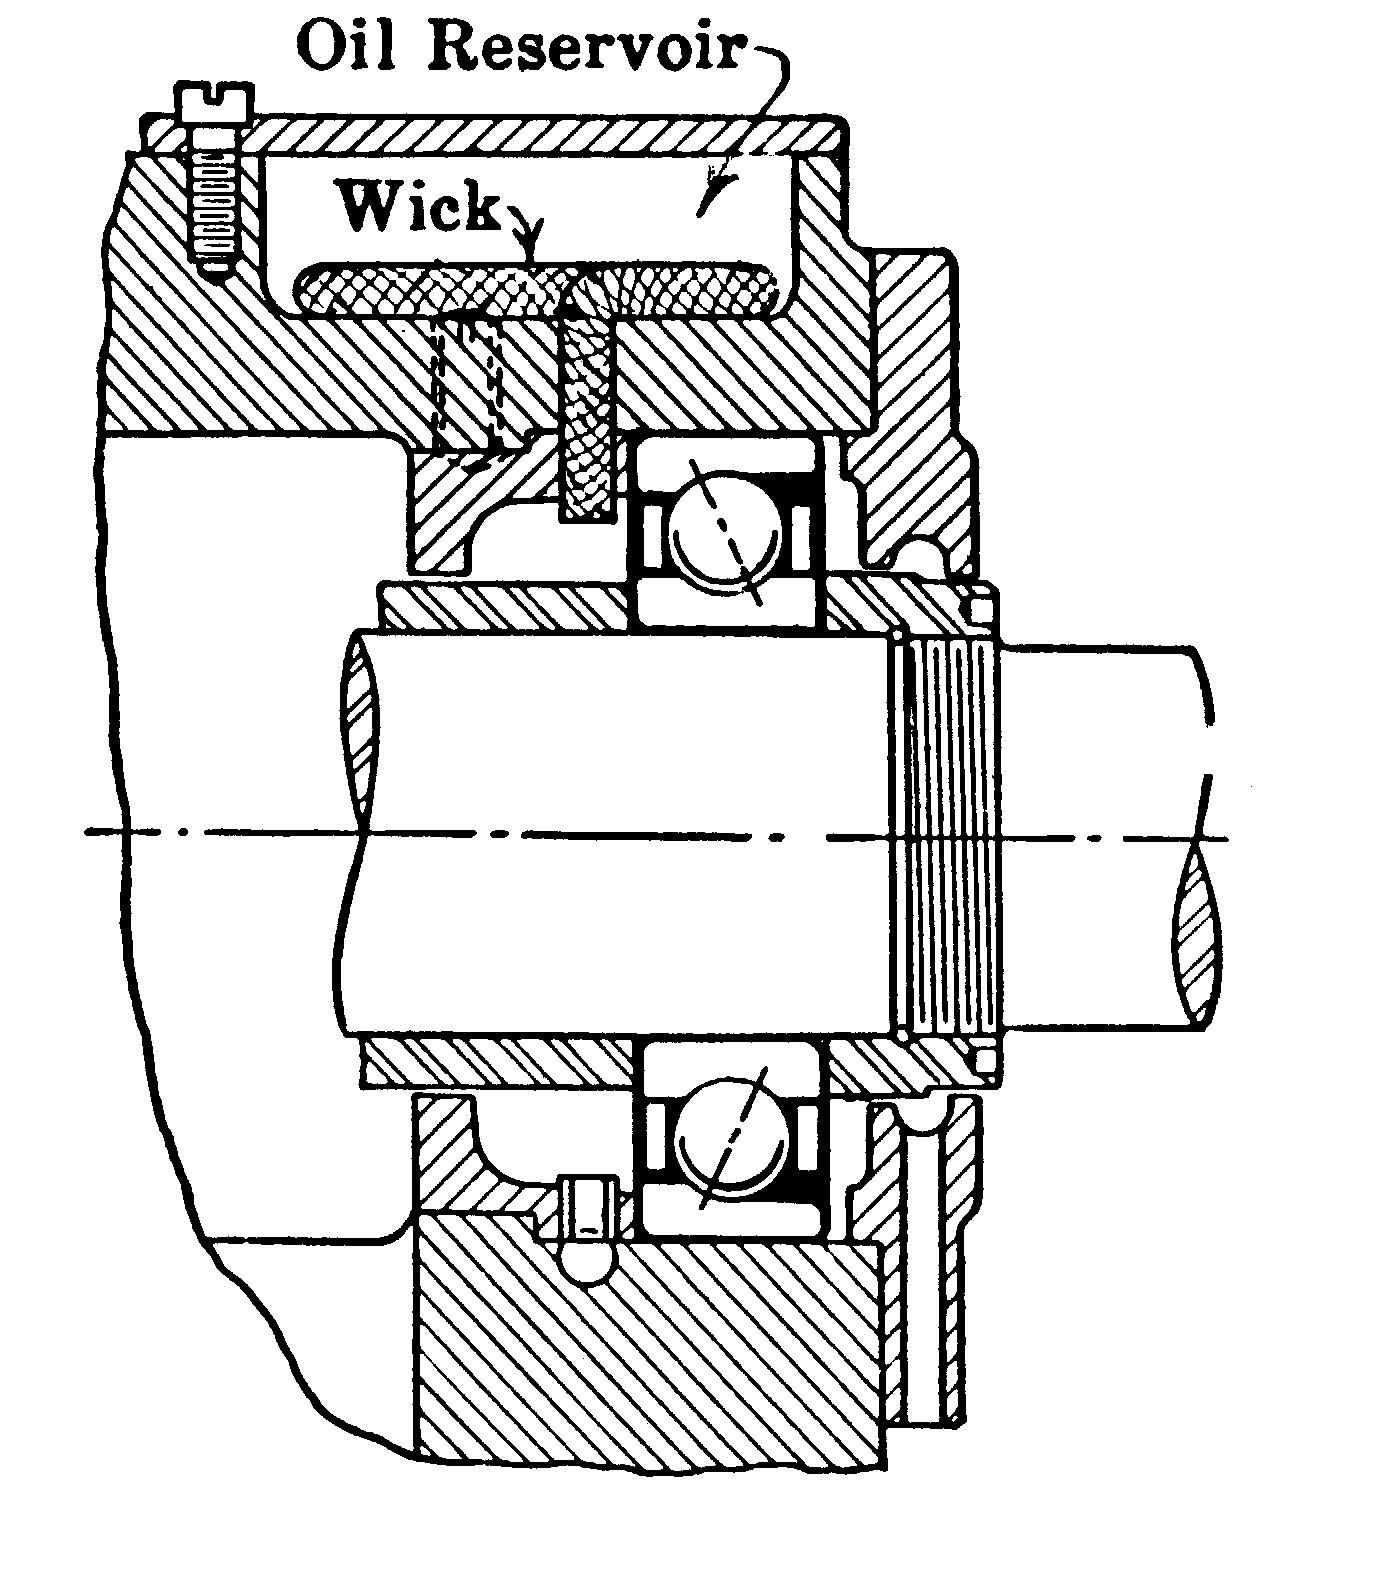
\includegraphics[width=.45\textwidth]{ball-bearing-2} 
\\
  (c) & (d)
\end{tabular}
%
\caption{Diverse Maschinenelemente als Beispiel für eine
Abbildung mit mehreren Elementen.
\emph{Overhang Mounting}~(a), \emph{Straddle Mounting}~(b),
einreihiges Rollenlager~(c), Schmierung von Rollenlagern~(d).
Diese Abbildung verwendet eine gewöhnliche Tabelle (\texttt{tabular}) mit
2 Spalten und 4 Zeilen (Details finden sich im Quelltext).
Bildquelle~\cite{Faires1934}.}
\label{fig:Bearings}
\end{figure}




\section{Tabellen}

Tabellen werden häufig eingesetzt um numerische Zusammenhänge, Testergebnisse
etc.\ in übersichtlicher Form darzustellen.
Ein einfaches Beispiel ist Tab.~\ref{tab:processors}, der \latex-Quelltext dazu
findet sich in Prog.~\ref{prog:processors-source}.


\begin{table}
\caption{Prozessor-Familien im Überblick.}
\label{tab:processors}
\centering
\setlength{\tabcolsep}{5mm}	% separator between columns
\def\arraystretch{1.25}			% vertical stretch factor (Standard = 1.0)
\begin{tabular}{|r||c|c|c|} \hline
& \emph{PowerPC} & \emph{Pentium} & \emph{Athlon} \\
\hline\hline
Manufacturer & Motorola & Intel & AMD \\
\hline
Speed & high & medium & high   \\
\hline
Price & high & high   & medium \\
\hline
\end{tabular}
\end{table}

\begin{program}
% place caption consistently either at the top or bottom:
\caption{\latex\ Quelltext zu Tab.~\ref{tab:processors}.
Die Erzeugung des dargestellten Listings selbst ist in Abschn.\ \ref{sec:programmtexte} beschrieben.}
\label{prog:processors-source}
%
\begin{LaTeXCode}[numbers=none]
\begin{table}
	\caption{Prozessor-Familien im Überblick.}
	\label{tab:processors}
	\centering
	\setlength{\tabcolsep}{5mm}	% separator between columns
	\def\arraystretch{1.25}		% vertical stretch factor
	\begin{tabular}{|r||c|c|c|} 
		\hline
		& \emph{PowerPC} & \emph{Pentium} & \emph{Athlon} \\
		\hline
		\hline
		Manufacturer & Motorola & Intel & AMD \\
		\hline
		Speed & high & medium & high   \\
		\hline
		Price & high & high   & medium \\
		\hline
	\end{tabular}
\end{table}
\end{LaTeXCode}
%
\end{program}

Manchmal ist es notwendig, in Tabellen relativ viel Text in engen Spalten
unter zu bringen, wie in Tab.~\ref{tab:synthesis-techniques}. In diesem Fall
ist es sinnvoll, auf den Blocksatz zu verzichten und gleichzeitig die
strengen Abteilungsregeln zu lockern. Details dazu finden sich im zugehörigen
\latex-Quelltext.


%--------------------------------------------------------------------------------
% Table with narrow columns
%--------------------------------------------------------------------------------
\begin{table}
\caption{Beispiel für eine Tabelle mit mehrzeiligem Text in engen Spalten.
Hier werden die Zeilen für den Blocksatz zu kurz, daher wird linksbündig
gesetzt (im "`Flattersatz"').}
\label{tab:synthesis-techniques}
\centering
\def\rr{\rightskip=0pt plus1em \spaceskip=.3333em \xspaceskip=.5em\relax}
\setlength{\tabcolsep}{1ex}
\def\arraystretch{1.20}
\setlength{\tabcolsep}{1ex}
\small
\begin{english}
\begin{tabular}{|p{0.2\textwidth}|c|p{0.3\textwidth}|p{0.2\textwidth}|}
\hline
   \multicolumn{1}{|c}{\emph{Method}} &
   \multicolumn{1}{|c}{\emph{Implem.}} &
   \multicolumn{1}{|c}{\emph{Features}} &
   \multicolumn{1}{|c|}{\emph{Status}} \\
\hline\hline
   {\rr polygon shading} &
   SW/HW &
   {\rr flat-shaded polygons} &
   \\
\hline
  {\rr flat shading with z-buffer} &
  SW/HW &
  {\rr depth values} &
  \\
\hline
  {\rr goraud shading with z-buffer} &
  SW/HW &
  {\rr smooth shading, simple fog, point light sources} &
  {\rr SGI entry models} \\
\hline
  {\rr phong shading with z-buffer} &
  SW/HW &
  {\rr highlights} &
  \\
\hline
  {\rr texture mapping with z-buffer} &
  SW/HW &
  {\rr surface textures, simple shadows} &
  {\rr SGI high end, flight simulators} \\
\hline
%  {\rr reflection mapping with z-buffer} &
%  SW/HW &
%  {\rr reflections} &
%  {\rr SGI next generation} \\
%\hline
%  {\rr raytracing} &
%  SW &
%  {\rr refraction, real camera model, area light sources with penumbra, realistic material models} &
%  {\rr common ray\-tracers} \\
%\hline
%  {\rr raytracing + global illumination simulation} &
%  SW &
%  {\rr indirect illumination} &
%  \textit{Radiance} \\
%\hline
%  {\rr raytracing + global illumination simulation + dissipating media} &
%  none &
%  {\rr realistic clouds, scattering, ...} &
%  {\rr research} \\
%\hline
\end{tabular}
\end{english}
\end{table}

%--------------------------------------------------------------------------------



\section{Programmtexte}
\label{sec:programmtexte}

Die Einbindung von Programmtexten (source code) ist eine häufige Notwendigkeit,
\va natürlich bei Arbeiten im Bereich der Informatik.

\subsection{Formatierung von Programmcode}
\label{sec:FormatierungVonProgrammcode}

Es gibt für \latex\ spezielle Pakete zur Darstellung von Programmen, die \ua\ auch die automatische Nummerierung der Zeilen vornehmen, insbesondere das \texttt{listings}-Package.%
\footnote{\url{http://www.ctan.org/tex-archive/macros/latex/contrib/listings/}}
Damit sind auch die in Tabelle~\ref{tab:CodeUmgebungen} aufgelisteten Code-Umgebungen 
realisiert.
%
\begin{table}
\caption{In \nolinkurl{hgb.sty} vordefinierte Code-Umgebungen.}
\label{tab:CodeUmgebungen}
\centering
\begin{tabular}{llll}
	\hline
	C (ANSI): & \verb!\begin{CCode}! & \verb!...! \verb!\end{CCode}! \\
	C++ (ISO): & \verb!\begin{CppCode}! & \verb!...! \verb!\end{CppCode}! \\
	C\#: & \verb!\begin{CsCode}! & \verb!...! \verb!\end{CsCode}! \\
	CSS: & \verb!\begin{CssCode}! & \verb!...! \verb!\end{CssCode}! \\
	HTML: & \verb!\begin{HtmlCode}! & \verb!...! \verb!\end{HtmlCode}! \\
	Java: & \verb!\begin{JavaCode}! & \verb!...! \verb!\end{JavaCode}! \\
	JavaScript: & \verb!\begin{JsCode}! & \verb!...! \verb!\end{JsCode}! \\
	\latex: & \verb!\begin{LaTeXCode}! & \verb!...! \verb!\end{LaTeXCode}! \\
	Objective-C: & \verb!\begin{ObjCCode}! & \verb!...! \verb!\end{ObjCCode}! \\
	PHP: & \verb!\begin{PhpCode}! & \verb!...! \verb!\end{PhpCode}! \\
	Swift: & \verb!\begin{SwiftCode}! & \verb!...! \verb!\end{SwiftCode}! \\
	XML: & \verb!\begin{XmlCode}! & \verb!...! \verb!\end{XmlCode}! \\
	Generisch: & \verb!\begin{GenericCode}! & \verb!...! \verb!\end{GenericCode}! \\
	\hline
\end{tabular}
\end{table}
%
Die Verwendung ist äußerst einfach, \zB\ für Quellcode in der Programmiersprache C schreibt man
%
\begin{quote}
\begin{verbatim}
\begin{CCode}
    ... 
\end{CCode}
\end{verbatim}
\end{quote}
%
Der Quellcode innerhalb dieser Umgebungen wird in der jeweiligen Programmiersprache interpretiert, wobei Kommentare erhalten bleiben. Diese Umgebungen können sowohl alleinstehend (im Fließtext) oder innerhalb von Float-Umgebungen (insbes.\ \texttt{program}) verwendet werden. Im ersten Fall wird der Quelltext auch über Seitengrenzen umgebrochen. Mit \verb!/+! ... \verb!+/! ist eine Escape-Möglichkeit nach \latex\ vorgesehen, die \va\ zum Setzen von Labels für Verweise auf einzelne Programmzeilen nützlich ist, \zB\ mit
%
\begin{quote}
\verb!/+\label{ExampleCodeLabel}+/!
\end{quote}
%
Ein Beispiel mit Java ist in Prog.~\ref{prog:CodeExample} gezeigt, wobei der oben angeführte Label in Zeile \ref{ExampleCodeLabel} steht.
Man beachte, dass innerhalb der Kommentare auch mathematischer Text 
(wie etwa in Zeile \ref{MathInCode} von Prog.~\ref{prog:CodeExample}) stehen kann.


\subsubsection{Nummerierung der Code-Zeilen}

Alle in Tabelle~\ref{tab:CodeUmgebungen} angeführten Code-Umgebungen können
mit optionalen Argumenten verwendet werden, die insbesondere zur Steuerung der
Zeilennummerierung hilfreich. 
Im Normalfall (also ohne zusätzliche Angabe) mit
%
\begin{quote}
\verb!\begin{!\texttt{\emph{some}Code}\verb!} ... !
\end{quote}
%
werden alle Code-Zeilen (einschließlich der Leerzeilen) bei 1 beginnend und 
fortlaufend nummeriert.
%
Bei aufeinanderfolgenden Codesegmenten ist es oft hilfreich, die Nummerierung 
aus dem vorherigen Abschnitt kontinuierlich weiter laufen zu lassen,
ermöglicht durch die Angabe des optionalen Arguments 
\texttt{firstnumber={\obnh}last}:
%
\begin{quote}
\verb!\begin{!\texttt{\emph{some}Code}\verb!}[firstnumber=last] ... !
\end{quote}
%
Um die Nummerierung der Codezeilen gänzlich zu unterbinden genügt die Angabe
des optionalen Arguments
\texttt{numbers={\obnh}none}:
%
\begin{quote}
\verb!\begin{!\texttt{\emph{some}Code}\verb!}[numbers=none] ... !
\end{quote}
%
In diesem Fall ist natürlich die Verwendung von Zeilenlabels im Code nicht
sinnvoll.


\subsection{Platzierung von Programmcode}

Da Quelltexte sehr umfangreich werden können, ist diese Aufgabe nicht
immer leicht zu lösen. Abhängig vom Umfang und vom Bezug zum Haupttext
gibt es grundsätzlich drei Möglichkeiten zur Einbindung von Programmtext:
%
\begin{itemize}
\item[a)] im laufenden Text für kurze Programmstücke,
\item[b)] als Float-Element (\texttt{program}) für mittlere Programmtexte bis max.\ eine Seite oder
\item[c)] im Anhang (für lange Programmtexte).
\end{itemize}

\subsubsection{Programmtext im laufenden Text}

Kurze Codesequenzen können ohne weiteres im laufenden Text
eingebettet werden, sofern sie an den gegebenen Stellen von unmittelbarer
Bedeutung sind. Die folgende (rudimentäre) Java-Methode \texttt{extractEmail} sucht
nach einer E-Mail-Adresse in der Zeichenkette
\texttt{line}:
%
\begin{JavaCode}[numbers=none]
static String extractEmail(String line) {
    line = line.trim(); // find the first blank
    int i = line.indexOf(' '); 
    if (i > 0)
        return line.substring(i).trim();
    else
        return null;
}
\end{JavaCode}
\medskip

\noindent
Dieses Codestück wurde mit 
%
\begin{quote}
\begin{verbatim}
\begin{JavaCode}[numbers=none]
static String extractEmail(String line) {
    line = line.trim(); // find the first blank
    ...
}
\end{JavaCode}
\end{verbatim}
\end{quote}
%
erstellt (siehe Abschn.\ \ref{sec:FormatierungVonProgrammcode}). 
In-line Programmstücke sollten maximal einige Zeilen lang sein und 
nach Möglichkeit nicht durch Seitenumbrüche geteilt werden.
%Um auch längere Programmzeilen unterzubringen, empfiehlt es sich, dafür
%eine entsprechend kleine Schriftgröße zu wählen (als Standardgröße ist
%\texttt{footnotesize} eingestellt). 


\subsubsection{Programmtexte als Float-Elemente}
Sind längere Codesequenzen notwendig, die in unmittelbarer Nähe des laufenden Texts
stehen müssen, sollten diese genauso wie andere Abbildungen als Float-Elemente
behandelt werden. Diese Programmtexte sollten den Umfang von einer Seite nicht übersteigen.
Im Notfall können auch bis zu zwei Seiten in aufeinanderfolgende Abbildungen gepackt werden,
jeweils mit eigener Caption. In \texttt{hgb.sty} ist eine neue Float-Umgebung \texttt{program} definiert, die analog zu \texttt{table} verwendet wird:
%
\begin{quote}
\begin{verbatim}
\begin{program}
\caption{Der Titel zu diesem Programmstück.}
\label{prog:xyz}
\begin{JavaCode}
  class IrgendWas {
    ...
  }
\end{JavaCode}
\end{program}
\end{verbatim}
\end{quote}
%
Wenn gewünscht, kann die Caption auch unten angebracht werden 
(jedenfalls aber konsistent und nicht gemischt).
Natürlich darf auch hier nicht mit einer linearen Abfolge im fertigen
Druckbild gerechnet werden, daher sind Wendungen wie
"`... im  folgenden Programmstück ..."' zu vermeiden und entsprechende Verweise
einzusetzen. Beispiele sind Programme \ref{prog:processors-source} und \ref{prog:CodeExample}.

\begin{program}
% place caption consistently either at the top or bottom:
\caption{Beispiel für die Auflistung von Programmcode als Float-Element.}
\label{prog:CodeExample}
\begin{JavaCode}
import ij.ImagePlus;
import ij.plugin.filter.PlugInFilter;
import ij.process.ImageProcessor;

public class My_Inverter implements PlugInFilter {
	int agent_velocity;
  String title = ""; // just to test printing of double quotes

	public int setup (String arg, ImagePlus im) {
		return DOES_8G;	// this plugin accepts 8-bit grayscale images /+\label{pr:IjSamplePlugin10}+/
	}

	public void run (ImageProcessor ip) {
		int w = ip.getWidth();	/+\label{ExampleCodeLabel}+/
		int h = ip.getHeight(); 
		
		/* iterate over all image coordinates */
		for (int u = 0; u < w; u++) { 
			for (int v = 0; v < h; v++) {
				int p = ip.getPixel(u, v); 
				ip.putPixel(u, v, 255-p); // invert: /+$I'(u,v) \leftarrow 255 - I(u,v)$\label{MathInCode}+/
			}
		}
	}		
} // end of class My_Inverter
\end{JavaCode}
%
\end{program}


\subsubsection{Programmtext im Anhang}

Für längere Programmtexte, speziell wenn sie vollständige
Implementierungen umfassen und im aktuellen Kontext nicht
unmittelbar relevant sind, muss zur Ablage in einem getrennten
Anhang am Ende des Dokuments gegriffen werden. Für Hinweise auf bestimmte
Details können entweder kurze Ausschnitte in den laufenden Text
gestellt oder mit entsprechenden Seitenverweisen gearbeitet werden. Ein
solches Beispiel ist der \latex-Quellcode in Anhang
\ref{app:latex} (Seite \pageref{app:latex}).%
\footnote{%
Grundsätzlich ist zu überlegen, ob die gedruckte Einbindung der gesamten
Programmtexte einer Implementierung für den Leser überhaupt sinnvoll ist, oder
ob diese nicht besser elektronisch (auf Datenträger) beigefügt und nur exemplarisch
beschrieben werden.}
